\section{Explicabilidade Causal}

\begin{frame}{Explicabilidade Causal}{De volta à Hierarquia de Pearl}
    Lembra da Hierarquia Causal? \pause O nível 3, \textit{counterfactual}, pergunta ``e se eu tivesse agido diferente?''. 

    É exatamente a pergunta que aparece quando alguém quer entender (ou contestar) uma decisão automatizada.

    \pause
    \vfill
    Duas famílias de explicação, duas perguntas bem diferentes:
    \begin{itemize}
        \item \textbf{SHAP} (atribuição): ``o que pesou nessa previsão?'';
        \pause
        \item \textbf{DiCE} (contrafactual): ``o que eu precisaria mudar pra mudar o resultado?''.
    \end{itemize}
\end{frame}

\begin{frame}{Explicabilidade Causal}{SHAP vs. Contrafactual, num exemplo real}
    \begin{columns}[T]
        \begin{column}{0.52\textwidth}
            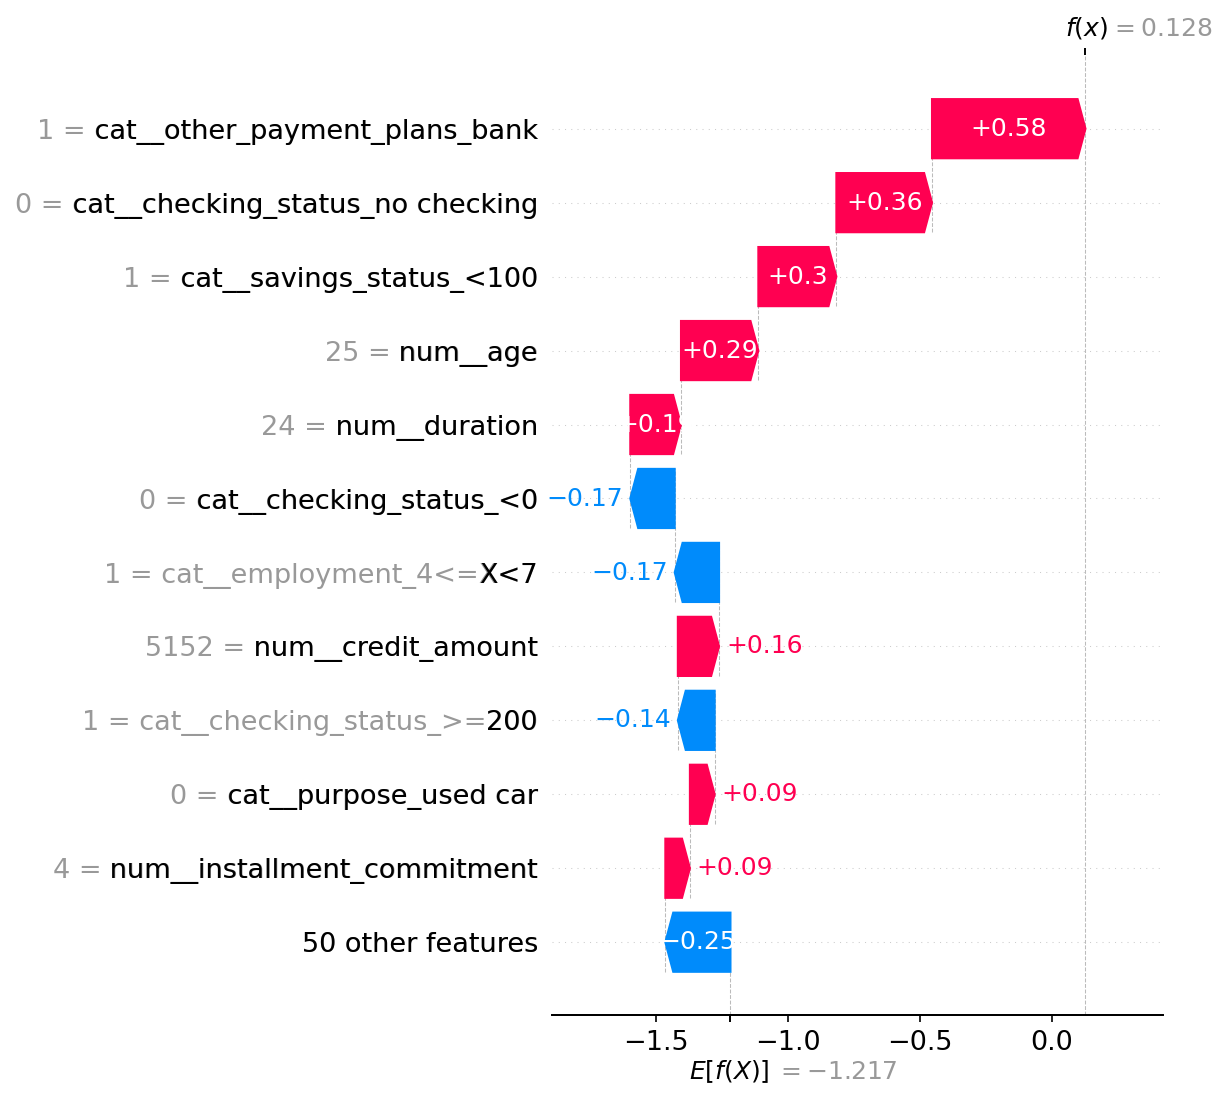
\includegraphics[width=\linewidth]{figures/7_shap_waterfall.png}
        \end{column}
        \begin{column}{0.48\textwidth}
            Esse é um SHAP \textit{waterfall} de um pedido de crédito negado.

            \vspace{10pt}
            Ele diz o que ``pesou'' na decisão do modelo... \pause mas não diz o que fazer a respeito.

            \pause
            \vspace{10pt}
            E se um dos atributos que mais pesou for algo que a pessoa não pode simplesmente mudar (idade, nacionalidade)?
        \end{column}
    \end{columns}
\end{frame}

\begin{frame}{Explicabilidade Causal}{Contrafactuais precisam de causalidade}
    Um gerador de contrafactuais sem nenhuma restrição pode sugerir ``mude sua idade de 25 pra 65'', o que é matematicamente válido, mas impossível na vida real.

    \pause
    \vfill
    A correção natural é usar o grafo causal: restringir a busca só a atributos \textit{mutáveis}, e propagar mudanças pelos seus efeitos causais (ex: aumentar o tempo de emprego também deveria mudar a renda esperada).

    \pause
    \vfill
    É a mesma lição do curso inteiro, aplicada em outro lugar: \textbf{o grafo carrega as suas suposições}, e ignorá-lo tem custo prático, não só teórico.

    \begin{alertblock}{Notebook extra!}
		Caso queira aprofundar nesse assunto, veja o notebook extra \#6.
	\end{alertblock}
\end{frame}
